\chapter{Threat Model}
\label{ch:ThreatModel}
\section{Contextual Theat Model}
\begin{figure}
  \centering
  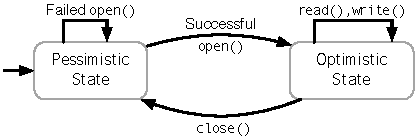
\includegraphics[width=\columnwidth]{fig/state-machine.pdf}
  \caption{A finite-state machine view of Trusted Capsule's threat model. Each
    capsule on a device begins in the pessimistic state. A successful transition
    from the pessimistic to optimistic state means an app on the device tried to
    open the capsule and the capsule's policy authorized the access. Only that
    app process is allowed to access that file in the optimistic state. When the
    the process closes the file, the system transitions back to the pessimistic
    state.}
  \label{fig:threatmodelstatediag}
\end{figure}

Trusted Capsules use a threat model that changes based on the context in which the application is executing. As illustrated in
Figure~\ref{fig:threatmodelstatediag}, this model has two states, {\em
  pessimistic} and {\em optimistic}, and there is a transition between
the two states depending on the context. We assume that device owners
have full control over the software stack running in the normal world
but may not modify the stack running within TrustZone.

The system begins in the {\em pessimistic} state when the user first receives a
capsule, which is encrypted data bundled with a policy that
governs its access. In this state, the TCB consists solely of ARM TrustZone and
the secure monitor; the OP-TEE OS running in TrustZone; the Trusted Capsules
data monitor that runs in OP-TEE OS. All code running outside of TrustZone
(i.e., the normal world kernel and apps) are considered untrusted. In this
state, we guarantee that the capsule's decrypted contents are not available and
that it is safe from attempts to either exfiltrate or modify its data or
policies. When the user opens the capsule with an app (which will use the {\tt
  open()} syscall), the policy embedded in the capsule is executed by the
Trusted Capsules data monitor. If the policy denies access to the file, the
system remains in the pessimistic state (and the app's call to {\tt open()} will
fail).

If access is allowed, the system transitions to the {\em optimistic} state where
the decrypted capsule data is given to the app. The TCB in this state expands to
include the normal world kernel and the app that opened the file. Only that app
is authorized to access the file and we rely on the process isolation mechanisms
in the normal world kernel to prevent other unauthorized apps from accessing the
decrypted data. When the app closes the file (with the {\tt close()} syscall),
the capsule is re-sealed and the system transitions back to the pessimistic
state. If the app modifies the file before closing it, the changes are saved
only if allowed by the capsule policy. Otherwise, they are discarded and the capsule is resealed with the original capsule data.

We consider side-channel and analog attacks out-of-scope. We can not control the application from transmitting the capsule's decrypted contents during the optimistic state of operation.

% We consider out-of-scope side-channel and analog attacks, and buggy or malicious
% capsule policies.

\section{Discussion}

% \iv{I would lead with the table and describe each scenario in the context of
%   the relevant table cell.}
%
% \ar{Done.}

% \iv{I would move the table higher, and also not have it break up the
%   flow of your scenario.}
%
% \ar{Done.}

\begin{table}[ht]
  \small
  \begin{center}
    \begin{tabular}{|l|l|l|} \hline
      \diagbox{{\bf Adversary}}{{\bf State}}& Pessimistic & Optimistic \\
      \hline
      Weak& \Checkmark& \Checkmark \\
      \hline
      Strong& \Checkmark& \XSolid \\
      \hline
    \end{tabular}
  \end{center}
  \caption{An enumeration of the possible system state and adversary type
    combinations. The \Checkmark \ and \XSolid \ symbols indicate whether or not
    Trusted Capsules prevents data exfiltration in the corresponding
    scenario. Note that the adversary here is not authorized to directly open a
    capsule on the device.}
  \label{tab:trustedcapprot}
\end{table}

Table~\ref{tab:trustedcapprot} summarizes the protections Trusted Capsules
offers depending on the adversary's capabilities and the state of the
system. Consider the scenario when Alvin sends a capsule with a photo to
Barbara's smartphone with a policy that requires Barbara to authenticate herself
before she can view the photo. In the worst case, Barbara herself is an
adversary interested in leaking the photo. There are no mechanisms in Trusted
Capsules preventing Barbara from doing so; the best that can be done is for Alvin to
be sure he trusts Barbara before he authorizes her to view the photo.

Consider instead the situation where Barbara is trustworthy but her smartphone
is sometimes accessible by Charlie, an adversary who is secretly interested in
viewing Alvin's photo. Charlie aims to modify the state of the smartphone so
that when Barbara subsequently regains control of her phone and opens Alvin's
capsule, Charlie surreptitiously receives a copy of the photo.

If the system is in the pessimistic state, there is no way for Charlie to view
the photo because the capsule is sealed and encrypted. In the optimistic state,
whether Charlie can exfiltrate the photo depends on whether he is a {\em weak}
or a {\em strong} adversary. A weak adversary is one who is not technically
inclined and hence may not do much more than install new apps from the
smartphone app store. In this event, when Barbara opens the capsule and the
system switches to the optimistic state, Trusted Capsules relies on the kernel's
app isolation mechanisms to prevent other unauthorized apps Charlie might have
installed from accessing the decrypted capsule data.

On the other hand, if Charlie is a strong adversary, then he may use a variety of
techniques such as kernel modifications to access the photo in the optimistic
state. While Trusted Capsules does not protect against this scenario at the
moment, it may be mitigated by having the policy reason about the normal world
software stack before opening the capsule. We leave an investigation of this
strategy to future work. Finally, note that regardless of the system state and
adversary type, an adversary may not alter the policy embedded in a capsule and
it never leaves the TrustZone environment.

% \iv{I think the state machine view that we drafted on the whiteboard
%  is missing to connect the 'transition' between these. i.e., the
%  'states' are actual states in a state machine. I think we need to
%  add the FSM to make this more clear. It will also help the
%  description above.}
%
% \ar{Added the state diagram above. Hopefully, this makes the explanation
%  clearer.}
